\chapter{Introduction}

	
	
	% \begin{figure}[H]
	%\includegraphics[width=13cm,height=5cm]{/Users/Whosham/Desktop/ICT/report/PIC/3.png}
	%\caption{Let's Encrypt vs Commercial Certificate Authorities}
	%\end{figure}
	 
	 
	\section{Abstract}

The Blockchain technology is having a huge potential since it had a huge contribution in redefining the way the data is stored, updated, and moved.
it is expected that the blockchain will revolutionize different business and industry. with such huge capabilities,
In this report, we proposed a platform for detecting fake news using Hypereledger fabric technology, we implemented an android application in order to, help the users to share and rank nearby events. Thanks to Hyperledger fabrics' features like immutability, trustworthy, transparency, we proposed a prototype of our application to mitigate the spread of fake news our application leveraging the blockchain technology and enabling it as a simple use case in the industry.\newline 

This report describes the proposed work as follow, we will start with a walk through the application and the use case scenario, in chapter 2 we will give a brief introduction about blockchain and Hyperledger fabric. In chapter 3 we discuss the application infrastructure we used, for instance, the network nodes, SDK implementation, and API calls. In Chapter 4 we are summarizing the android application part and how we designed and developed the application in depth. Chapter 5 will focus on the results and insights gained in a performance evaluation.
\cleardoublepage

	\section{Introduction Walk-Through}
	The spread of social media and integrating it as an essential part of our daily life has a tremendous effect on spreading fake news. Many adults prefer getting news from the social media platforms like Facebook and Twitter more than the legacyways like newspaper and broadcast, with the advance of technology it become trivial to manipulate images and videos.   
	Our mission is to mitigate fake news with our platform we incent users to publish and rank nearby events based on their reputation. By using hyperledger technology it will be hard to manipulate the data once it's stored on the blockchain.\\ we are using a ranking scheme to increase the trustworthiness of the users, by virtue of the chain code or smart contract, which will be responsible for handling the business logic and rank the events based on users location and  trustworthiness. The architecture of our application could be described in particular as below: 	 

       \begin{enumerate}
	 \item {A User can capture an event or text and upload it using our android application to the blockchain.}
	 \item {The event's data will be stored permanently on the blockchain and it will be impossible to be altered.} 
	 \item {Our application will fetch and display the events to the nearby users.} 
         \item {The users in the area will be able to judge the events and upload comments and further media files that approve or disapprove the events.  we are restricting the participation of the users in judging events only legitimate users that their locations are in the nearby area will be eligible to vote \footnote[1]{collecting time and location evidence in order to assure that the users were in the nearby area and their location wasn't spoofed  is part of a separate bachelor thesis running in parallel.} }
         \item {Depending on the other users reviews the event received, the chain code will update the trustworthiness value of the event \footnote[2]{Ranking the trustworthiness of the events and the users will be based on the reviews of the event in addition to the trusted code execution is part of a separate thesis running in parallel. } }
          \item {The chain code will update the user's score based on the reviews that his events received in another word the reviews of the events will directly affect the user reputation for example, An event which received good reviews will increase the user's reputation and gives him more score and credits on our platform.} 
	\end{enumerate}
	In \hyperref[fig:appflow]{Figure 1} we described the previously mentioned procedures as an overview of our platform.
	\begin{figure}[H]
	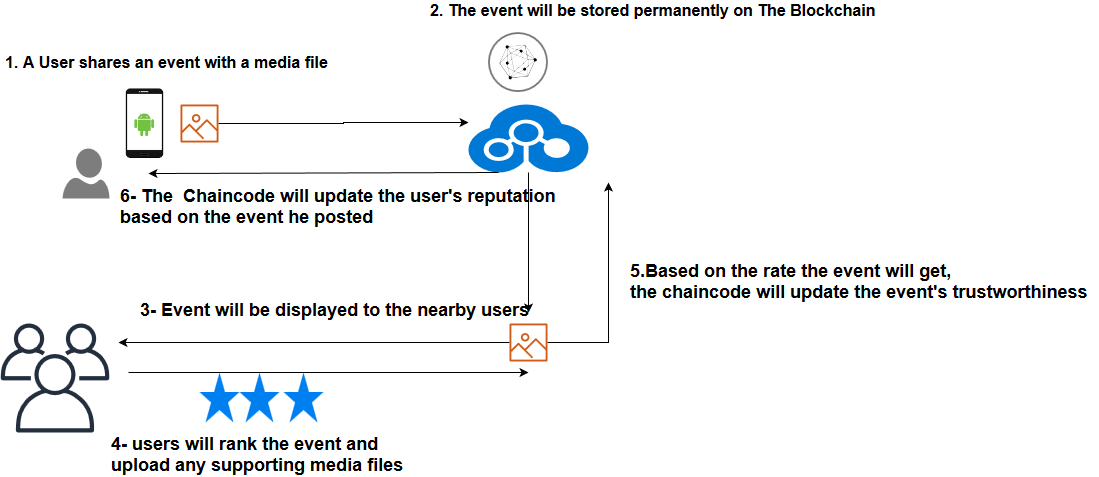
\includegraphics[width=15cm,height=5cm]{images/appflow.png}
	\caption{The Application Walkthrough}
	\label{fig:appflow}
	\end{figure}

\section{Architecture}
The platform would be dismantled into three main components: 
\begin{itemize}
  \item The Hyperledger fabric network.
  \item The Backend and Fabric SDK. 
  \item The Android Development. 
\end{itemize}

We will discuss every single component in details in a separate chapter we will start with the necessary background information about the Blockchain and main components and terms of hyper ledger fabric for example peers, chaincode, transaction ..etc. \\ Then we will discuss the backend, API Design  and how the API call requests will be consumed and the nodejs SDK handles the request, then forwards it to the chaincode which is the only way to interact with the blockchain.
Finally, we will discuss the Android application design, UI elements , network request in json that is calling API and the coding in depth with all the functions implemented \hyperref[fig:architecture]{Figure 2} depicts all the architecture overview of the platform. 
\begin{figure}[H]
	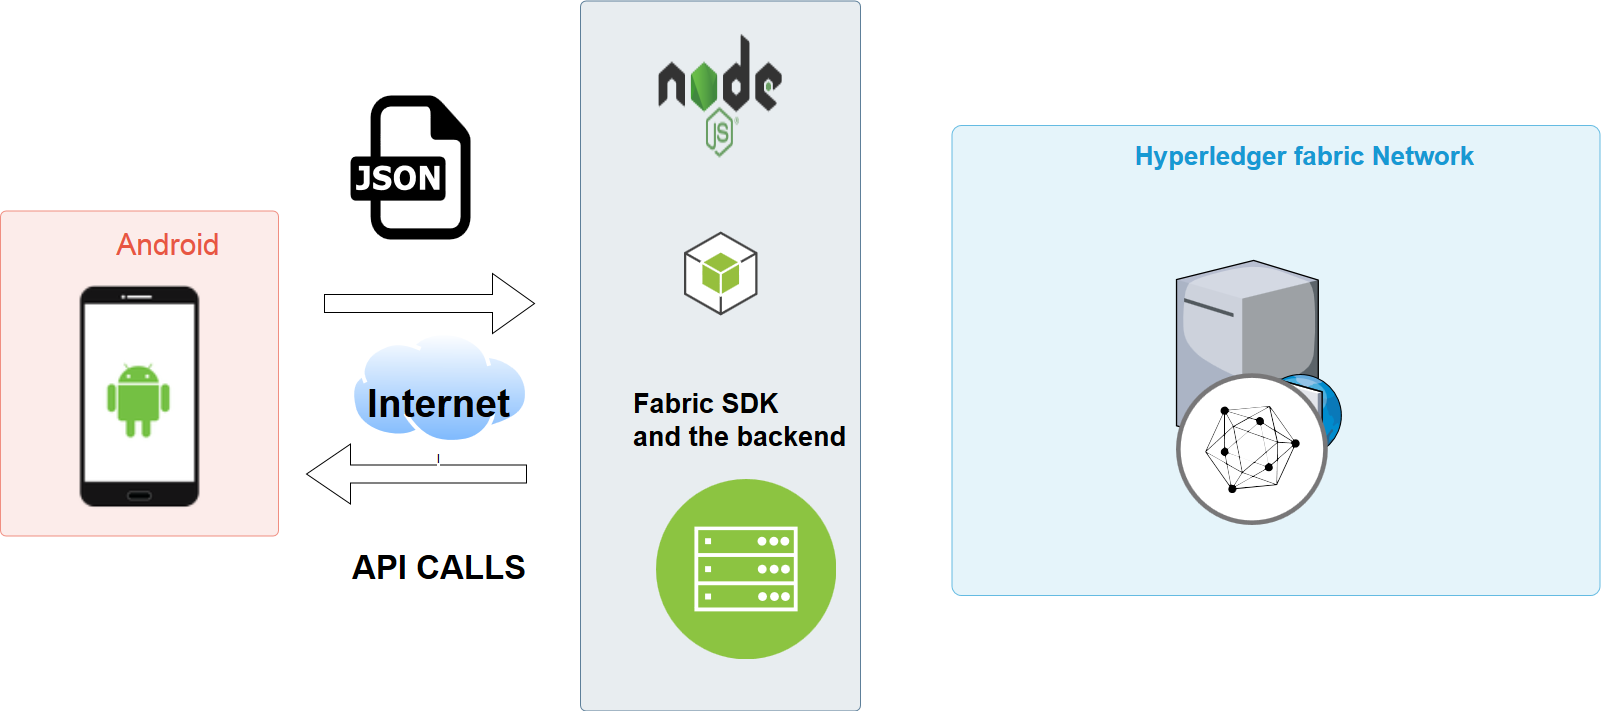
\includegraphics[width=15cm,height=10cm]{images/architecture.png}
	\caption{Architecture Overview}
	\label{fig:architecture}
	\end{figure}

      

 


      